\section{Introduction}
\label{sec:introduction}
To place our study in context we discuss the relevance of post-starburst galaxies in the broader field of galaxy evolution. We then focus upon the characteristics of PSBs: their spectra, morphology and their relationship to major mergers. There are two main themes to our research: kinematic position angle analysis of velocity fields, and Radon transforms of stellar velocity fields, both of which will be introduced in due course.

\subsection{Galaxy evolution and PSBs}
\label{sec:evolution}
Galaxies are the building blocks of the universe. We strive to understand how galaxies form and evolve. In this project we investigate the evolutionary pathways of a specific subset of galaxies, post-starburst galaxies, which ceased star-formation about 1 to 2 Gyr ago, to determine if there is evidence of past major mergers that may have caused this  shutdown in star-formation activity.

Current theories of galaxy evolution are often presented and explained  by referring to galaxy colour-colour and colour-magnitude diagrams (CMD) \citep[see e.g.][]{2001AJ....122.1861S, 2003ApJ...585L...5H, 2003ApJS..149..289B,baldry2004quantifying,2006MNRAS.373..469B}. A representative CMD constructed from Sloan Digital Sky Survey SDSS-IV MaNGA observations of nearby galaxies (z < 0.04) is presented in  Figure~\ref{fig:CMD-G_i-i}. The CMD exhibits a strong colour-magnitude bimodality features.  Gas-rich, star-forming, generally late-type galaxies, Sb, Sc and Irregular, populate the so-called blue cloud region of the CMD. As gas is consumed through star formation blue cloud galaxies are understood to transition to the redder mainly early-type E, S0 and Sa quiescent galaxies along the upper left in the red sequence region of the CMD. There is a sparsely populated region separating the blue cloud and red sequence populations referred to as the green valley \citep{2004ApJ...608..752B}. In this project we explore the evolutionary pathway of galaxies that are in transition from the blue cloud to the red sequence, through the green valley.

\begin{figure}
    \centering
    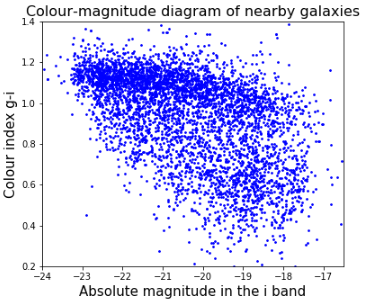
\includegraphics[width=\columnwidth]{images/CMDs/CMD-G_i-i.png}
    \caption[SDSS-IV MaNGA galaxy colour-magnitude diagram]{SDSS-IV MaNGA galaxy colour-magnitude diagram: the distribution of nearby galaxies from the Sloan Digital Sky Survey data release DR15. The colour index g-i is plotted against the i-band magnitude M$_i$. The distribution exhibits clear bimodality with mainly late-type galaxies occupying the blue cloud in the lower right while early-type galaxies form a red sequence along the upper region of the diagram extending to brighter magnitudes. There is a sparsely populated band separating the two densely populated regions, the so-called 'green valley'.}
    \label{fig:CMD-G_i-i}
\end{figure}

Another useful visualisation of the distribution of local galaxies takes the form of a colour-mass diagram: here we use the colour index ratio of near-ultraviolet to infrared (NUV-i) flux plotted against log stellar mass. The colour-mass distribution of all galaxies in the MaNGA data release 15 (DR15) dataset is presented in Figure \ref{fig:CMD-mass-1}. This colour-mass diagram also reveals the densely populated blue cloud region, in this case in lower left, and the red red sequence in the upper right. These over-dense features are visually enhanced where the density contour lines\footnote{\href{https://seaborn.pydata.org/generated/seaborn.kdeplot.html}{Contour plot generated using the SciPy KDE (kernel density estimator) package.}} are tightly packed. We will use colour-mass diagrams later to illustrate the location of our subject PSB galaxies in colour-mass parameter space.

\begin{figure}
    \centering
    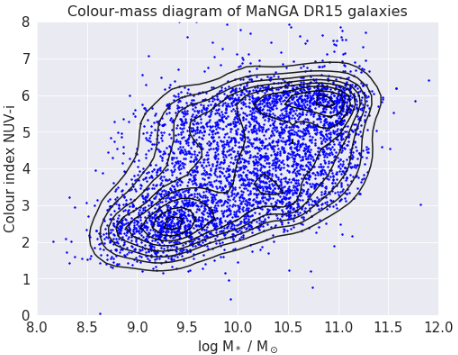
\includegraphics[width=\columnwidth]{images/CMDs/CMD-DR15-ALL-15.png}
    \caption[Colour-mass diagram of the complete MaNGA DR15 galaxy population]{An alternative representation of galaxy property distribution: colour index versus stellar mass. The plot portrays the distribution of colour index NUV-i versus log of stellar mass extracted from SDSS-IV MaNGA DR15 data. Contours of equal number density are overlaid on the scatter plot representation of individual galaxies. The density contours emphasis the locations of the blue cloud (lower left), red sequence (upper right) and the intervening sparsely populated green valley regions. }
    \label{fig:CMD-mass-1}
\end{figure}

\subsection{Post starburst galaxies: spectra, morphology and mergers}
\label{post-starburst-galaxies}
Post-starburst (PSB) galaxies are a class of galaxies that experienced an intense burst of star formation over one gigayear ago. Their spectra reveal that star formation has since ceased. There is no spectral evidence of young O- and B-type stars, even the least massive B stars created in the starburst will have gone supernova within the dynamical time since the  event. PSB spectra are dominated by strong Balmer absorption lines, H$\beta$, H$\gamma$ and H$\delta$. Strong Balmer lines reveal a present population of main sequence A- and F-type stars \citep{1997A&A...325.1025P}. In contrast, nebular emission is an indicator of ongoing star formation, for example the emission lines H$\alpha$ 6564 \AA\ and [OII] 3727\AA, but such emission line features are weak or absent in PSBs. Weak nebular emission coupled with strong Balmer absorption features are characteristic of galaxies that have evolved since sustaining a starburst phase in the past 1 to 2 Gyr \citep{2001ApJ...547L..17B,2003PASJ...55..771G,2004MNRAS.355..713B,2005MNRAS.357..937G,2018MNRAS.477.1708P}. These spectral observations are characteristic of a brief burst of star formation in the past which has subsequently ceased, or been 'quenched' \citep{1983ApJ...270....7D,1987MNRAS.229..423C,1997A&A...325.1025P}. The presence of such spectral features are indicative that PSB galaxies are in transition on an evolutionary track from blue, active star-forming disc galaxies, to redder passive spheroids \citep{2004MNRAS.355..713B,2012MNRAS.420..672S,2013MNRAS.429.2212M}. 

Morphology describes the shape and structural appearance of galaxies. The morphology of PSBs is consistent with early-type ellipticals and therefore PSBs are alternatively referred to as E+A (elliptical morphology plus A-type stars) or k+A galaxies \citep{1983ApJ...270....7D,1996ApJ...466..104Z,2009ARA&A..47..159B}. Using a sample of low-redshift (z \textless\ 0.1) E+A galaxies from the 2dF Galaxy Redshift Survey (2dFGRS) \citet{2004MNRAS.355..713B} found morphological evidence of major mergers, such as tidal tails, and concluded that major mergers are an important formation mechanism for E+A post-starburst galaxies. More recent studies have shown that about half of nearby galaxies have experienced recent rapid quenching while on an evolutionary track to the red sequence \citep{Martin_2007,10.1111/j.1365-2966.2009.14537.x,2015MNRAS.450..435S}, however see \cite{2017ApJ...845..145W}. 

Quenching during mergers is also apparent in numerical simulations, see e.g. \cite{2019MNRAS.484.2447D}. \citet{2019NatAs...3..440P} report on evolutionary modelling simulations of PSB/E+A galaxies. They identify two distinct evolutionary pathways transitioning from the blue cloud to the red sequence. Both pathways reveal a phase of quenching caused by mergers.

Traditionally, identification of galaxy mergers has been carried out by visual classification of images. The Galaxy Zoo (GZ)\footnote{\href{http://zoo1.galaxyzoo.org/}{http://zoo1.galaxyzoo.org/}} project \citet{10.1111/j.1365-2966.2008.13689.x,10.1111/j.1365-2966.2010.17432.x, 2017MNRAS.464.4176W} engaged hundreds of thousands of 'citizen scientists' in an online census to perform morphological classification of one million galaxies by inspecting images from the SDSS. The project aimed primarily to classify galaxies visually to the Hubble sequence based on their morphology. An additional objective was to identify signs of merger processes. The GZ project identified evidence of mergers in 1 to 3\% galaxies in the local universe.

\cite{2016MNRAS.456.3032P} describe the morphological indicator designated 'shape asymmetry' for automated identification of galaxies exhibiting faint asymmetric tidal features indicative of ongoing or past mergers in order to determine whether PSBs play a transitory role in the buildup of the red sequence. \cite{2011arXiv1102.0550B} developed numerical simulations to explore the sensitivity of galaxy mass ratio in the detection of major mergers in starburst galaxies. Adopting a similar but more extensive approach, \cite{2019ApJ...872...76N} developed a merger classification scheme that can be applied directly to SDSS images. Their method is based on hydrodynamical and N-body models of mergers, which were then trained on model SDSS images. They find their method is sensitive to mass ratio, and major mergers are also sensitive to asymmetry. In a progression of that earlier work  \cite{2019DDA....5020304N} have extended the SDSS image classification method to incorporate kinematic predictors derived from MaNGA stellar velocity maps. This is the first merger classification scheme that utilises both imaging and kinematics. The authors will apply the technique to explore how star formation rates change with different stages and types of merger. 

In another approach, some researchers are applying Machine Learning or Deep Learning techniques to preexisting morphological catalogues in order to automate the identification of mergers. \citet{2018MNRAS.476.3661D} employed visual classification of SDSS images, obtained from the Galaxy Zoo 2 project (GZ2), combined this with machine learning algorithms based on convolutional neural networks (CNNs), to produce a reliable catalogue of  morphological classifications. Transfer learning using Deep CNN algorithms were used by \citet{2018MNRAS.479..415A} specifically targeting mergers. 

In this study we are concerned with the analysis of kinematic properties of post-starburst galaxies. The objective is to identify inherent signatures of past merger events. Major mergers may have caused quenching of star formation, triggering the PSB features and established their evolutionary tracks through the green valley towards the red sequence. 

\subsection{Structure of the paper}
The content of the project report is now organised as follows: Details of the MaNGA survey and the selection criteria for our PSB sample and associated control galaxies are provided in Section \ref{sec:data}. The two main themes of our kinematic data analysis are presented in separate sections: the kinematic position angle  analysis method is presented in Section \ref{sec:methods-I-kinemetry}, while Section \ref{sec:methods-II-Radon} describes the Radon transform method. Details of our research results from each of the two methods are presented in Section \ref{sec:results}. Salient points from the research results and the conclusions drawn from this work are discussed in Section \ref{sec:discussion} which includes some recommendations for future work.
